\documentclass[10pt]{article}

\usepackage[margin=1.5in]{geometry}
\usepackage{graphicx}
\usepackage{natbib}
%correct punctuation for MBE
\bibpunct[,]{(}{)}{;}{a}{}{,}
\usepackage{tablefootnote}
\usepackage{amsmath}

\renewcommand{\bottomfraction}{.9}
\renewcommand{\topfraction}{.9}
\renewcommand{\textfraction}{0.1}
\renewcommand{\floatpagefraction}{.9}

\linespread{1.5}
\begin{document}

\title{\textbf{Limited utility of residue masking in positive-selection inference}}
\author{Stephanie J. Spielman$^{1*}$ and Eric T. Dawson$^{1}$ and Claus O. Wilke$^{1}$}
\date{}

\maketitle
\noindent
Address:\\
$^1$Department of Integrative Biology, Center for Computational Biology and Bioinformatics, and Institute of Cellular and Molecular Biology.
The University of Texas at Austin, Austin, TX 78731, USA.\\

\bigskip
\noindent
$^*$Corresponding author\\
$\phantom{^*}$Email: stephanie.spielman@utexas.edu\\

\bigskip
\noindent
Manuscript type: research article

\bigskip
\noindent Keywords: multiple sequence alignment, alignment filters, positive-selection inference, sequence simulation

\newpag
\begin{abstract}
 Recent studies have noted that errors in multiple sequence alignments have the potential to reduce accuracy in positive-selection inference. It has therefore been suggested that alignments be filtered before further analyses \textbf{ <-I think passive might work better for that sentence, oddly}. One widely-used filter, known as Guidance, generates position-based confidence scores for a given alignment using a bootstrap approach, thereby allowing users to remove positions of low confidence from the alignment. Here, we have reimplemented the Guidance software to include two novel algorithms for phylogenetically correcting confidence scores. We additionally introduced a new score-normalization scheme which assigned lower scores to highly-gapped alignment columns. Using a sequence simulation approach, we compared our reimplemented Guidance algorithms to the original. We found, surprisingly, that no approach examined could substantially improve positive-selection inference across multiple inference methods, including PAML and FUBAR. Instead, it seemed that the analysis methods used influenced positive-selection inference substantially more than did filtering alignments with a Guidance-based strategy.
\end{abstract}


\section*{Introduction}
Constructing a multiple sequence alignment represents the first step of analysis in most studies of molecular evolution, namely phylogenetic reconstruction and evolutionary rate inference. Recently, several studies have shown that poor alignment quality can significantly hinder accuracy in such downstream analyses \citep{Jordan2012, MarkovaRaina2011, Dwivedi2009, Talavera2007, Ogden2006}. In particular, using low-quality alignments to infer positive selection elevated false positive rates \citep{Schneider2009, Fletcher2010, MarkovaRaina2011}. As a consequence, some studies have advocated applying an alignment filter to MSAs \citep{Jordan2012, Privman2012}. Such filters, which include Guidance \citep{Penn2010, Privman2012}, GBLOCKS \citep{Castresana2000}, and T-Coffee \citep{Notredame2000}, locate putatively poorly-aligned regions in alignments so that users can curate their alignments to maximize signal. The hope is that culling unreliable positions and/or columns from alignments will yield increased accuracy in positive-selection inference without excessively sacrificing power.

Of these filters, Guidance \citep{Penn2010} is currently the most widely used in positive-selection inference. Guidance derives a confidence score for each alignment position by sampling variants in the guide tree used to construct progressive alignments. Users can mask positions with scores below a given threshold, thereby removing residues that cannot be confidently placed in the alignment. This method is fairly conservative, as particular positions of low confidence can be removed rather than entire columns. Additionally, recent simulation studies have demonstrated that filtering poorly aligned residues with Guidance may increase accuracy when inferring positive selection \citep{Jordan2012,Privman2012}. 

However, while \citet{Privman2012} found dramatic improvements in positive-selection inference when applying the Guidance filter, a comprehensive study by \citet{Jordan2012} on alignment methods and filtering found that Guidance affected this inference modestly, if at all. In particular, they reported that, at lower protein divergence levels or insertion/deletion (indel) rates, Guidance neither substantially improved nor worsened positive-selection detection. Alternatively, at high divergence levels (1.8 mean-path-length, defined as mean root-to-tip branch length) or indel rates (0.2 indel/substitution events), \citet{Jordan2012} found that Guidance strongly boosted true positive rates. While these results were compelling, protein sequences used in positive selection studies rarely, if ever, contain sequences separated by such high divergences; for example, a typical mammalian gene tree's mean-path-length is only about 0.17 \citep{Spielman2013}, 10\% the divergence level at which Jordan and Goldman detected improvements when using the Guidance filter.

Motivated by these apparent discrepancies, we sought to determine whether altering the Guidance scoring algorithm could improve positive-selection inference at more realistic divergences. To this end, we reimplemented the Guidance software (see Methods for details) and examined the effects of novel scoring algorithms, which account for the sequences' phylogenetic relationships. We additionally implemented a new score-normalization scheme which naturally gave lower scores to residues in highly-gapped columns, which may contain more errors than regions with few gaps, to account for their inherent unreliability.

Using our reimplementation, we filtered alignments produced from realistic protein-coding sequence simulations and subsequently inferred positive selection with two methods: the recently-described FUBAR \citep{Murrell2013} and the current standard of use, the PAML M8 model \citep{Yang2007}. Overall, we found that neither the original Guidance filter nor our newly implemented filters conferred any substantial benefits to positive-selection inference, and any improvements recovered were of extremely small magnitude. Instead, the inference method used had a much greater effect on positive-selection detection.


\section*{Results}

\subsection*{Guidance reimplementation and analysis pipeline}
To systematically evaluate Guidance's influence on positive-selection inference, we reimplemented the Guidance software in Python and C++. Before conducting any analyses, we verified that, given a set of perturbed alignments, our program produced the same confidence scores as the original Guidance. In addition to our basic Guidance reimplementation, we derived two new algorithms, described in depth in Methods, which employ phylogenetic weighting when assigning confidence scores. Briefly, the first method incorporated a weight for each sequence in the alignment, as calculated by BranchManager \citep{Stone2007}, and the second method incorporated patristic distances (the sum of branch lengths between two taxa). We called these methods, respectively, BMweights and PDweights.  We additionally defined a ``gap-penalization" score-normalization scheme, which assigned scores scaled by a column's gappiness. In other words, this scheme naturally gave lower scores to highly-gapped columns, accounting for the fact that such regions were more likely to be poorly aligned. We referred to filters using the gap-penalization scheme as GuidanceP, BMweightsP, and PDweightsP.

We began by simulating 100 realistic protein-coding sequences using Indelible \citep{Fletcher2009} along each of four different gene trees of sizes 11, 26, 60, and 158 taxa. To ensure that these simulations produced real sequence data to the extent possible, we simulated according to evolutionary parameters inferred from H1N1 influenza hemagluttinin (HA), a protein well known to contain positively selected regions \citep{Bush1999, Kryazhimskiy2008, Meyer2012}. We then processed the unaligned sequences with our Guidance reimplementation using the aligner MAFFT L-INS-I (linsi) \citep{Katoh2005}. We chose to use only linsi, because it strongly outperforms other progressive alignment softwares for protein alignments \citep{Thompson2011,Nuin2006} without sacrificing speed. We scored each alignment using each of our three scoring algorithms (original Guidance, BMweights, and PDweights) with each of our two normalization schemes (original Guidance and gap-penalization). In all cases, we masked positions with scores below 0.5, the same threshold as used by \citet{Jordan2012}, with ``?".

Finally, we assessed positive selection with both the recently-described FUBAR \citep{Murrell2013} as implemented in HyPhy \citep{Pond2005} and the widely-used M8 model in PAML \citep{Yang2007}. Note that we use PAML throughout this paper to refer specifically to the M8 model.  All phylogenies used during these inferences were constructed from unfiltered amino-acid alignments in RAxML \citep{Stamatakis2006} using the CAT model under the WAG substitution matrix. All filtered alignments stemming from the same unfiltered alignment were analyzed with the same phylogeny to remove any potential bias that distinct phylogenies could introduce.We considered sites as positively selected if the given method returned a posterior probability $\geq0.90$. Note that, while we processed all alignments with FUBAR, we did not infer positive selection for the largest simulation set with PAML due to prohibitive runtimes. 


\subsection*{Filtering with Guidance-based methods has a minimal effect on positive-selection inference}

We then assessed how filtering alignments with a Guidance-based method influences positive-selection detection by comparing the resulting true positive rates (TPRs) of positive-selection inference between all filtered alignments and their corresponding unfiltered alignments. TPRs were derived using the true evolutionary rates assigned during sequence simulation (see Methods for details). We chose to primarily compare the TPRs as opposed to the false positive rates (FPRs), as FPRs were exceedingly small, never exceeding an average of 0.017 across simulation sets and methods. These FPRs were similar to those recovered by \citet{Jordan2012}. 

We first compared the two normalization schemes, original and gap-penalization, to one another for each of the three algorithms (Guidance, BMweights, and PDweights) examined. To this end, we built linear models, using the difference in average TPR between normalization schemes as the response and algorithm as a fixed effect (Table \ref{tab:penalmodel}) for each simulation set and inference method. Note that only filtered alignments were considered in these models. In all instances in which we detected a significant difference between normalization schemes, the gap-penalization scheme outperformed the original Guidance scheme, albeit by very small magnitudes. Therefore, we proceeded to compare the TPRs from gap-penalization algorithms (GuidanceP, BMweightsP, PDweightsP) to those of unfiltered alignments with a series of mixed-effects models. These models included TPR as the response variable, simulation count as a random effect, to account for the paired structure of our analysis, and algorithm as a fixed effect. Table \ref{tab:casemodel} gives the results from these models for each simulation set and selection inference method.

Overall, we did not recover any difference in TPR among filtering algorithms; Guidance and the two phylogenetically-weighted methods performed statistically indistinguishably for a given simulation set. Figure \ref{roc} displays ROC curves for positive-selection inference with FUBAR and PAML. Figures \ref{roc}B and \ref{roc}C specifically highlight the effect of alignment filtering with FUBAR and PAML, respectively, at low FPRs; for each respective method, areas under the unfiltered alignment curves were essentially the same as for the filtered alignment curves.

When processed with FUBAR, alignment filtering did significant increase the average TPR for the 60 and 158-sequence simulation sets. Even so, the magnitude of its improvements were very small, boosting unfiltered the average TPR by 0.03 for the 60-sequence set and 0.01 for the 158-sequence set. In other words, TPR increased on average by 10\% for the 60-sequence simulation set and by 3\% for the 158-sequence simulation set. Filtering neither improved nor worsened positive-selection inference for the 11 or 26-sequence simulation sets as analyzed with FUBAR.

Analyzing the data with PAML similarly did not result in a significant TPR change for the 11-sequence simulation set. Unlike when analyzing with FUBAR, we did not recover significant change in mean TPR change for the 60-sequence simulation set. Alternatively, PAML results showed that filtering did improve TPRs in the 26-sequence simulation set, albeit by an average of 4.68\%. While statistically significant, an increase of this low a magnitude may not have any noticeable effect on positive-selection inference in studies of real sequences. 

\subsection*{Influence of posterior probability on selection inference methods}

Our analysis recovered several differences in how PAML and FUBAR behaved when assessing positive selection. In particular, whether FUBAR or PAML performed better depended on the number of sequences analyzed; FUBAR outperformed PAML for the two smaller simulation sets of 11 and 26-sequences, but PAML outperformed FUBAR for the 60-sequence simulation set (Table \ref{tab:casemodel}). We found that this trend resulted from the posterior probability threshold chosen to call sites as positively selected. Figure \ref{tprfpr} shows how the average TPR and FPR for unfiltered alignments behaved for two different simulation sets (26 and 60-sequence) across posterior probabilities. With regards to TPRs,
FUBAR generally performed better than PAML at lower posterior probabilities, whereas PAML outperformed FUBAR at high probabilities. As the number of sequences increased, the intersection between methods' TPRs shifted towards lower posterior probabilities. {\textbf I think passive better here too:} This shift was largely dictated by PAML's improved ability to call true positives with the inclusion of more sequences, given that FUBAR's relationship between posterior probability and TPR remained similar between the two simulation sets.  Filtering alignments affected these broad trends that FUBAR and PAML portrayed only marginally, if at all (Figure \ref{fulltpr}). Thus, the analysis method used affected positive-selection inference substantially more than did filtering  alignments with a Guidance-based method. 

The relationship between posterior probability and FPR, unlike that of TPR, was mostly consistent between simulation sets for both FUBAR and PAML. While PAML achieved FPRs of nearly zero essentially immediately for both the 26 and 60-sequence simulation sets, FUBAR approached a zero FPR more slowly, reaching zero around a posterior probability of 0.8 for each simulation set. As a typical study of positive selection would almost certainly use a posterior probability above at least 0.8, alignment filtering would likely not be able to substantially reduce FPR.

How TPR and FPR behaved for FUBAR and PAML evidenced the different approaches these methods employ to detect positive selection; while PAML's M8 model aims to identify precise $dN/dS$ value at each site in an alignment, FUBAR merely assesses whether a site is positively selected without attempting to assign a point estimate of $dN/dS$ to each position. Having fewer sequences in an alignment, therefore, hindered PAML's ability to determine site-based $dN/dS$ values, rendering its positive-selection inference worse than that of FUBAR. Increasing the number of sequences allowed for PAML to make more robust $dN/dS$ estimates, and therefore positive-selection inferences, while it has a relatively smaller effect on FUBAR's approximations.

\subsection*{Raising masking thresholds for gap-penalization algorithms may hinder positive-selection inference}

When filtering alignments with Guidance-based methods, one must select a specific score cutoff below which to mask residues. We chose to filter all residues with scores less than 0.5. However, it was possible that selecting a different threshold would have yielded different results, so we analyzed how changing this threshold might impact our findings. For this analysis, we considered only the Guidance and GuidanceP scoring schemes since our phylogenetically-corrected algorithms did not perform significantly differently. Using the same position confidence scores previously generated, we masked all alignments at the additional cutoffs of 0.3, 0.7 and 0.9. We then inferred positive selection for each masking threshold with FUBAR alone, whose rapid runtime (under 15 minutes per alignment) allowed for this larger-scale investigation. 

Similar to previous analyses, we built two mixed-effects linear models for each simulation set, with TPR as the response, masking cutoff as a fixed effect, and simulation count as the random effect, for Guidance and GuidanceP results each. Results showed that, for Guidance, all masking cutoffs yielded statistically similar TPRs (multiple comparisons gave all $P>0.06$) for a given simulation set. For GuidanceP, on the other hand, masking cutoffs 0.3, 0.5, and 0.7 gave statistically similar TPRs (all $P>0.45$), whereas using a masking cutoff of 0.9 always yielded significantly lower TPRs than the other cutoffs. Table \ref{tab:cutoffs} highlights this result, specifically comparing the cutoff of 0.5 to 0.9 for GuidanceP. Importantly, for the 60-sequence simulation set (for which we noted the maximum benefit of alignment filtering), masking at the stringent cutoff of 0.9 as opposed the more lenient 0.5 reduced the TPR by roughly 26\%. This extreme TPR decrease yielded an average TPR of 0.281 for alignments masked at 0.9, well below its corresponding average unfiltered TPR of 0.345 (Table \ref{tab:casemodel}). The gap-penalization normalization, therefore, had the potential to remove excessive amounts of information from alignments and worsen positive-selection detection. 

%%%%%%%%%%%%%%%%%%%     OLD TEXT WE MAY WANT TO KEEP AROUND IN CASE %%%%%%%%%%%%%%%%%%%
%ROC curves did not control for the posterior probability threshold employed to call sites as positively selected. In other words, a given point on an ROC curve could easily correspond to different posterior probability thresholds for filtered and unfiltered alignments. Thus, while useful in assessing theoretical performance, ROC curves did not capture the reality of data analysis and might actually have been misleading.
%%%%%%%%%%%%%%%%%%%%%%%%%%%%%%%%%%%%%%%%%%%%%%%%%%%%%%%%%%%%%%%%%%%%%%



\section*{Discussion}

We have conducted a simulation-based study to evaluate the how introducing phylogenetically-aware scoring algorithms into the Guidance alignment filter influenced the detection of positive selection in protein-coding sequences. Additionally, we tested a novel score-normalization method, which assigned inherently lower scores to highly-gapped alignment columns. We ensured that our simulations resembled real sequence data by simulating along real gene trees according to evolutionary parameters derived from the H1N1 influenza hemagluttinin (HA) protein. We inferred positive selection for all alignments using two methods: the recently introduced and very fast FUBAR \citep{Murrell2013} within the HyPhy package \citep{Pond2005} and the current standard for evolutionary rate inference, the PAML M8 model \citep{Yang2007}.

We found that, while the gap-penalization scheme marginally improved upon the original normalization method, incorporating phylogenetic information did not significantly change affect in such analyses. Moreover, filtering alignments with any Guidance-based method, including the original, did not substantially improve positive-selection inference under any circumstance. That the phylogenetically-weighted algorithms did not improve upon the original Guidance algorithm indicated the minimal benefits that filtering in this manner produced at all. Were the original Guidance to offer robust improvements in positive-selection detection, one might expect that our more statistically controlled approach would boost the method's performance. However, as we have found that masking individual positions in an alignment only marginally affected positive-selection inference in the first place, one might not expect the algorithmic changes we implemented might to have a dramatic effect.

While others \citep{Schneider2009, Fletcher2010, MarkovaRaina2011,Privman2012} have noted a prevalence of false positives in positive-selection inference of real sequence data, we recovered very low false positive rates. The FPRs we detected were very similar to those of  \citet{Jordan2012}, yet substantially lower than those detected by \citet{Privman2012}, the two studies which have previously investigated the specific utility of the Guidance filter \textbf{I feel like it's awkward to include the Privman given that I don't believe any of their results}. We attributed our small FPRs to the fact that we employed simulated sequences, which represents the only strategy to assess methodological accuracy with complete confidence.  We ensured realism in our sequence data by applying evolutionary parameters inferred from a very large HA alignment (1028 sequences), which previous studies have demonstrated to contain pervasive positive selection \citep{Bush1999, Kryazhimskiy2008, Meyer2012}. We chose to use HA as a reference for evolutionary parameters because of its wealth of sequence data; having such a large data set allowed for robust evolutionary inference and the assurance that our simulations mimicked realistic sequence data. However, rather than conduct our simulations along our HA phylogeny, we decided to evolve sequences along eukaryotic gene trees for tractability. Simulating along a phylogeny of over 1000 sequences would not represent an excessive computational burden, but a typical positive-selection study would likely not use this many sequences. Additionally, the most important aspect to consider when selecting a phylogeny along which to simulate sequences is the phylogeny's topology, and the gene trees we used were topologically typical of an evolutionary rate study.

In sum, our simulations indicated that, while alignment filtering offered some benefits, those improvements were marginal at best. With such minimal changes to positive-selection inference, alignment filtering could easily decrease accuracy in a given positive selection study. Indeed, we noted that using a stringent masking cutoff of 0.9 for algorithms normalized with our gap-penalization strategy resulted in extreme decreases in TPR relative to an unfiltered alignment. Choosing a low filtering threshold was necessary to achieve any improvement in positive-selection inference.  

Overall, we cannot unequivocally recommend the use of a Guidance-based alignment filter when inferring positive selection. Once an alignment has been constructed, it does not seem that much can be done to eliminate any misleading information. Instead, researchers should select inference methods in which the error can be minimized as much as possible without necessitating post-hoc correction. Therefore, we recommend that users select high-quality alignment and inference methods to minimize any obscuring signal, instead of relying on filters. If one must filter an alignment, we recommend using a lenient cutoff $\leq0.5$ to avoid sacrificing power, which might worsen inferences.


\section*{Methods}

\subsection*{Guidance Reimplementation}
Our reimplemented Guidance is written in Python and C++. Following the algorithm set forth in Penn et al. \citep{Penn2010}, we first create a reference amino-acid alignment using a user-specified progressive alignment software, with choices of Clustalw \citep{Thompson1994}, MUSCLE \citep{Edgar2004}, or MAFFT \citep{Katoh2002, Katoh2005}. We then generate $N$ (where $N=100$, by default) bootstrapped alignment replicates, each of which is used to create a bootstrapped tree in FastTree2 \citep{Price2010}. We then use these $N$ trees as guide trees to create $N$ new perturbed alignments, which we subsequently compare to the reference alignment to generate a confidence score for each residue. Users can specify options for aligner and phylogeny as desired.

\subsubsection*{Scoring Algorithms}
We additionally implemented two new scoring algorithms which incorporate phylogenetic information. Before calculating scores, a phylogeny is built from the reference alignment. Our program includes functionality to build this phylogeny using either either FastTree2 \citep{Price2010} or RAxML \citep{Stamatakis2006}. Again, users can specify options to the phylogenetic construction software selected. Using this phylogeny, two types of phylogenetic weights can be calculated. The first uses the software package BranchManager \citep{Stone2007} to calculate a weight for each taxon in the phylogeny representing that taxon's contribution to the phylogeny as a whole. We call this method ``BMweights." The second method calculates patristic distances (sum of branch lengths) between each taxon in the phylogeny using the python package DendroPy \citep{Sukumaran2010}. We call this method ``PDweights."

We calculate positional confidence scores for each of the $N$ bootstrap alignments as follows. A raw score, $S$, for a given residue in row $i$, column $j$ of the reference alignment is calculated as \begin{equation} S_{ij} = \sum\limits_{k \in R_{ng}^j} I_{ik}^j s_{ik}^j    ,\end{equation} where $R_{ng}^j$ represents all rows in column $j$ which are not gaps.
In this formula, the indicator function 
\begin{equation}I_{ik}^j = \left\{ \begin{array}{rl}

              1                         &\mbox{if reference alignment residue pair $(i, k)$ is present in bootstrap alignment} \\
              0            &\mbox{if reference alignment residue pair $(i, k)$ is absent in bootstrap alignment} \\
                     \end{array} \right. 
\end{equation}
serves to compare the bootstrap- and reference-alignment residue pairings.
We calculate $s_{ik}^j$ according to the given scoring algorithm:
\begin{equation}
s_{ik}^j = \left\{ \begin{array}{rl}

              1                         &\mbox{if Guidance} \\
              w_iw_k              &\mbox{if BMweights} \\
              d_p(i,k)              &\mbox{if PDweights} \\
                     \end{array} \right.,
\end{equation} where $w_i$ is the phylogenetic weight of the taxon at row $i$, as calculated by BranchManager, and $d_p(i, k)$ is the patristic distance between the taxa at rows $i$ and $k$. 

We then sum positional scores $S_{ij}$ determined from each bootstrap alignment and normalize them to yield a final score $\widetilde{S}_{ij}$ for each reference alignment residue. We use two different normalization schemes. The first scheme, given by \begin{equation} \widetilde{S}_{ij} = \frac{\sum_{n}^N S_{ij}(n)}{N\sum_{k \in R_{ng}^j} S_{kj}}, \end{equation} normalized by only considering the residue-residue comparisons made, as done by \citep{Penn2010}. The second scheme was given by 

\begin{equation} \widetilde{S}_{ij} = (\sum_N^n S_{ij}) \bigg/ \left\{ \begin{array}{rl}
              N\sum\limits_{k \in R_{all}}^j 1                                  &\mbox{if Guidance} \\
              N\sum\limits_{k \in R_{all}}^j d_p(i,k)                         &\mbox{if BMweights} \\
   		  Nw_i                                       &\mbox{if PDweights} \\          
         \end{array} \right.,
\end{equation}
where $R_{all}^j$ represents all rows in column $j$, including gap. This second normalization scheme naturally gives lower scores to highly gapped columns, and we therefore called it the ``gap-penalization" normalization. We refer to the algorithms normalized by the first scheme as Guidance, BMweights, and PDweights. When normalized with the gap-penalization scheme, we refer to them, respectively, as GuidanceP, BMweightsP, and PDweightsP. Note that scores calculated using the Guidance algorithm with the first normalization scheme are equivalent to those originally derived by \citet{Penn2010}. 



\subsection*{Sequence Simulation}
Coding sequences were simulated using Indelible \citep{Fletcher2009}. To ensure that our simulations reflected realistic protein sequences, we simulated according to evolutionary parameters of the H1N1 hemagluttinin (HA) influenza protein. To derive these parameters, we aligned 1028 HA protein sequences with linsi \citep{Katoh2005} and then back-translated to a codon alignment using the original nucleotide sequence data. We generated a phylogeny from this codon alignment in RAxML \citep{Stamatakis2006} using the GTRGAMMA model. Using the codon alignment and phylogeny, we inferred evolutionary parameters with the REL (random effects likelihood)  method \citep{NielsenYang1998} using the software HyPhy \citep{Pond2005}, with five evolutionary rate categories as free parameters under the GY94 evolutionary model \citep{GoldmanYang1994}. We employed a Bayes Empirical Bayes approach \citep{Yang2000} to obtain infer $dN/dS$ values at each site, which we used to assess a complete distribution of site rates. The resulting distribution was log-normal with a mean $dN/dS = 0.37$ with 8.3\% of sites  under positive selection ($dN/dS>1$). We binned these rates into 50 equally spaced categories for specification in Indelible, which required a discrete distribution of $dN/dS$ values. Again according to parameters derived from the HA analysis, we fixed $\kappa$, the transition-to-transversion ratio, at 5.3 for all simulations. We additionally set the state codon frequencies for our simulations according to those directly calculated from the HA alignment. 

We simulated 100 alignments across four different real gene trees each, yielding a total of 400 simulated alignments. Phylogenies used included an 11-taxon tree of the mammalian olfactory receptor OR5AP2 \citep{Spielman2013}, a 26-taxon tree of mammalian rhodopsin sequences \citep{Spielman2013}, a 60-sequence tree of phosphoribulokinase (PRK) genes from photosynthetic eukaryotes \citep{Yang2011}, and a 158-taxon multilocus tree of flatfish sequences \citep{Betancur2013}. The latter two phylogenies were obtained from TreeBase.
For each simulation set, we directly calculated an indel (insertion-deletion) rate directly from these trees’ original alignments, to use as simulation parameters, by dividing the total number of gaps present by the total number of positions in each alignment. Respectively, indel rates were 0.053, 0.019, 0.0041, and 0.0066. 

\subsection*{Alignment and Positive-Selection Inference}
We constructed all alignments using linsi \citep{Katoh2002,Katoh2005} within the context of our Guidance reimplementation. In addition to an unfiltered alignment, we generated six filtered alignments (one for each filtering algorithm and each normalization scheme), masking residues with scores below cutoffs of 0.3, 0.5, 0.7, and 0.9. We inferred positive selection for every condition using both FUBAR \citep{Murrell2013} with default parameters. We processed only the unfiltered alignments and alignments masked at a scoring cutoff of 0.5 with the PAML M8 model, specifying $F3\times4$ codon frequency and ``cleandata = 0" in the control file \citep{Yang2007}. Phylogenies specified for positive-selection inference were those constructed during the Guidance alignment procedure when deriving phylogenetic weights. All filtered alignments derived from a unfiltered alignment were processed with identical phylogenies to remove any confounding effects of differing phylogenies. Note that while we employed FUBAR to assess positive selection for all simulation sets, we did not use PAML to infer positive selection for the largest set (158 sequences).

We then compared resulting positive-selection inferences for each alignment to its respective true alignment's $dN/dS$ values, given by Indelible during simulation, to assess performance accuracy. As residues may have been differently aligned relative to the true simulated alignment, we adopted a consensus method to compare alignments we constructed to the true simulations. If at least 50\% of the residues present in a true alignment column were present in an inferred alignment column, we considered the true alignment column's $dN/dS$ as the true value forthat inferred alignment column. We considered sites positively selected if the posterior probability of $(dN/dS>1) \geq 0.9$.

Statistics were performed using Python and R. Linear modeling was conducted using the R packages lme4 \citep{Bates2012} and
multcomp \citep{Hothorn2008}. All code used is available at \textbf{the github or something}.



\begin{figure*}[H]
\centerline{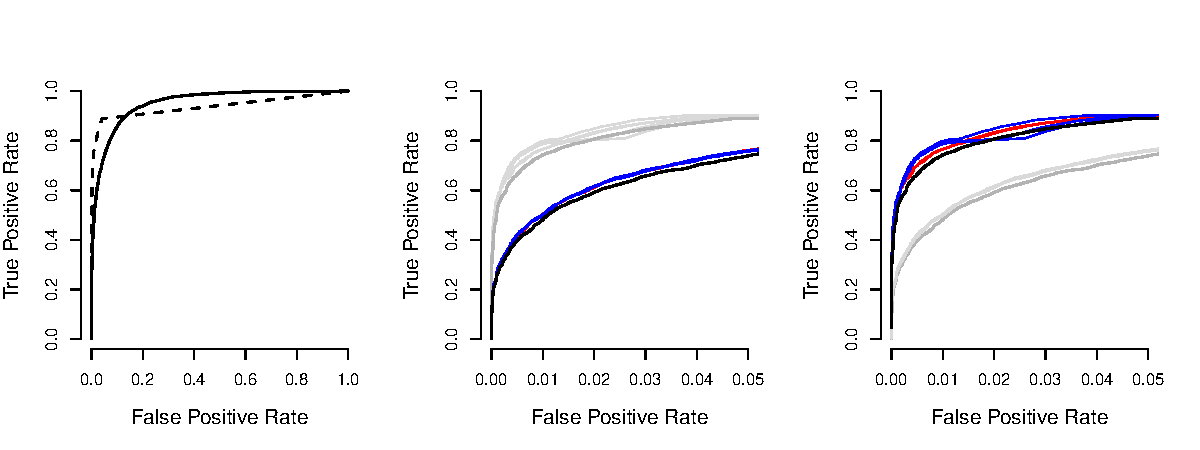
\includegraphics[width=7in]{Figures/roc.pdf}}
\caption{\label{roc} ROC curve as averaged across 60-sequence simulation set. A) Unfiltered alignments for FUBAR (solid) and PAML (dashed). Note that neither method achieved FPRs greater than shown. B) FUBAR in color with PAML results shown in grey. C) PAML in color with FUBAR results shown in grey.}
\end{figure*}



\begin{figure*}[H]
\centerline{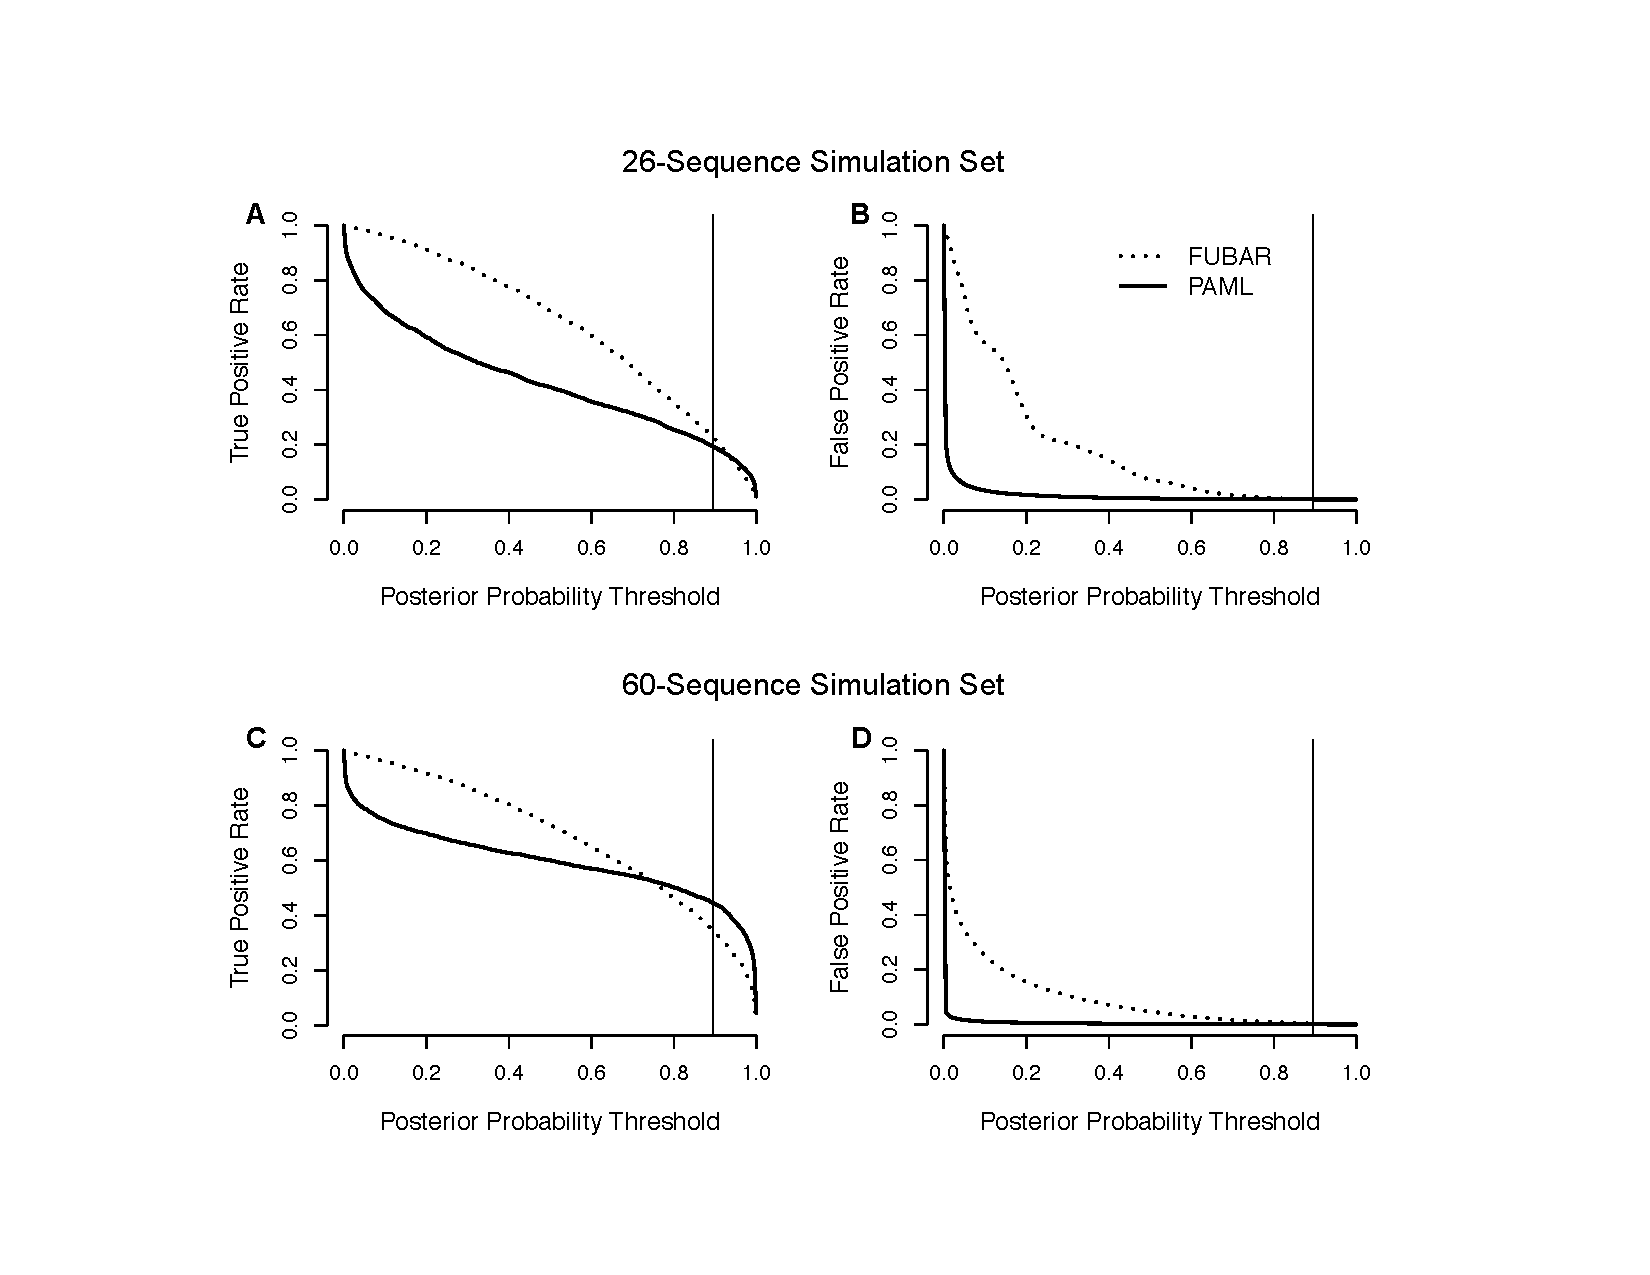
\includegraphics[width=7in]{Figures/tprfpr.pdf}}
\caption{\label{tprfpr} True and false positive rates recovered from FUBAR and PAML analysis with unfiltered alignments, averaged across the 26-sequence and the 60-sequence simulation sets, against the posterior probability threshold used to call sites as positively selected. A) TPR, 26-sequence set. B) FPR, 26-sequence set. C) TPR, 60-sequence set. D) FPR, 60-sequence set.  As the number of sequences increased, PAML's TPR improved at lower posterior probabilities, while its FPR remained remarkably low across all posterior probabilities for both simulation sets. While FUBAR's performance did improve with the inclusion of more sequences, its overall TPR behavior did not change as dramatically as did PAML's.}
\end{figure*}



\begin{figure*}[H]
\centerline{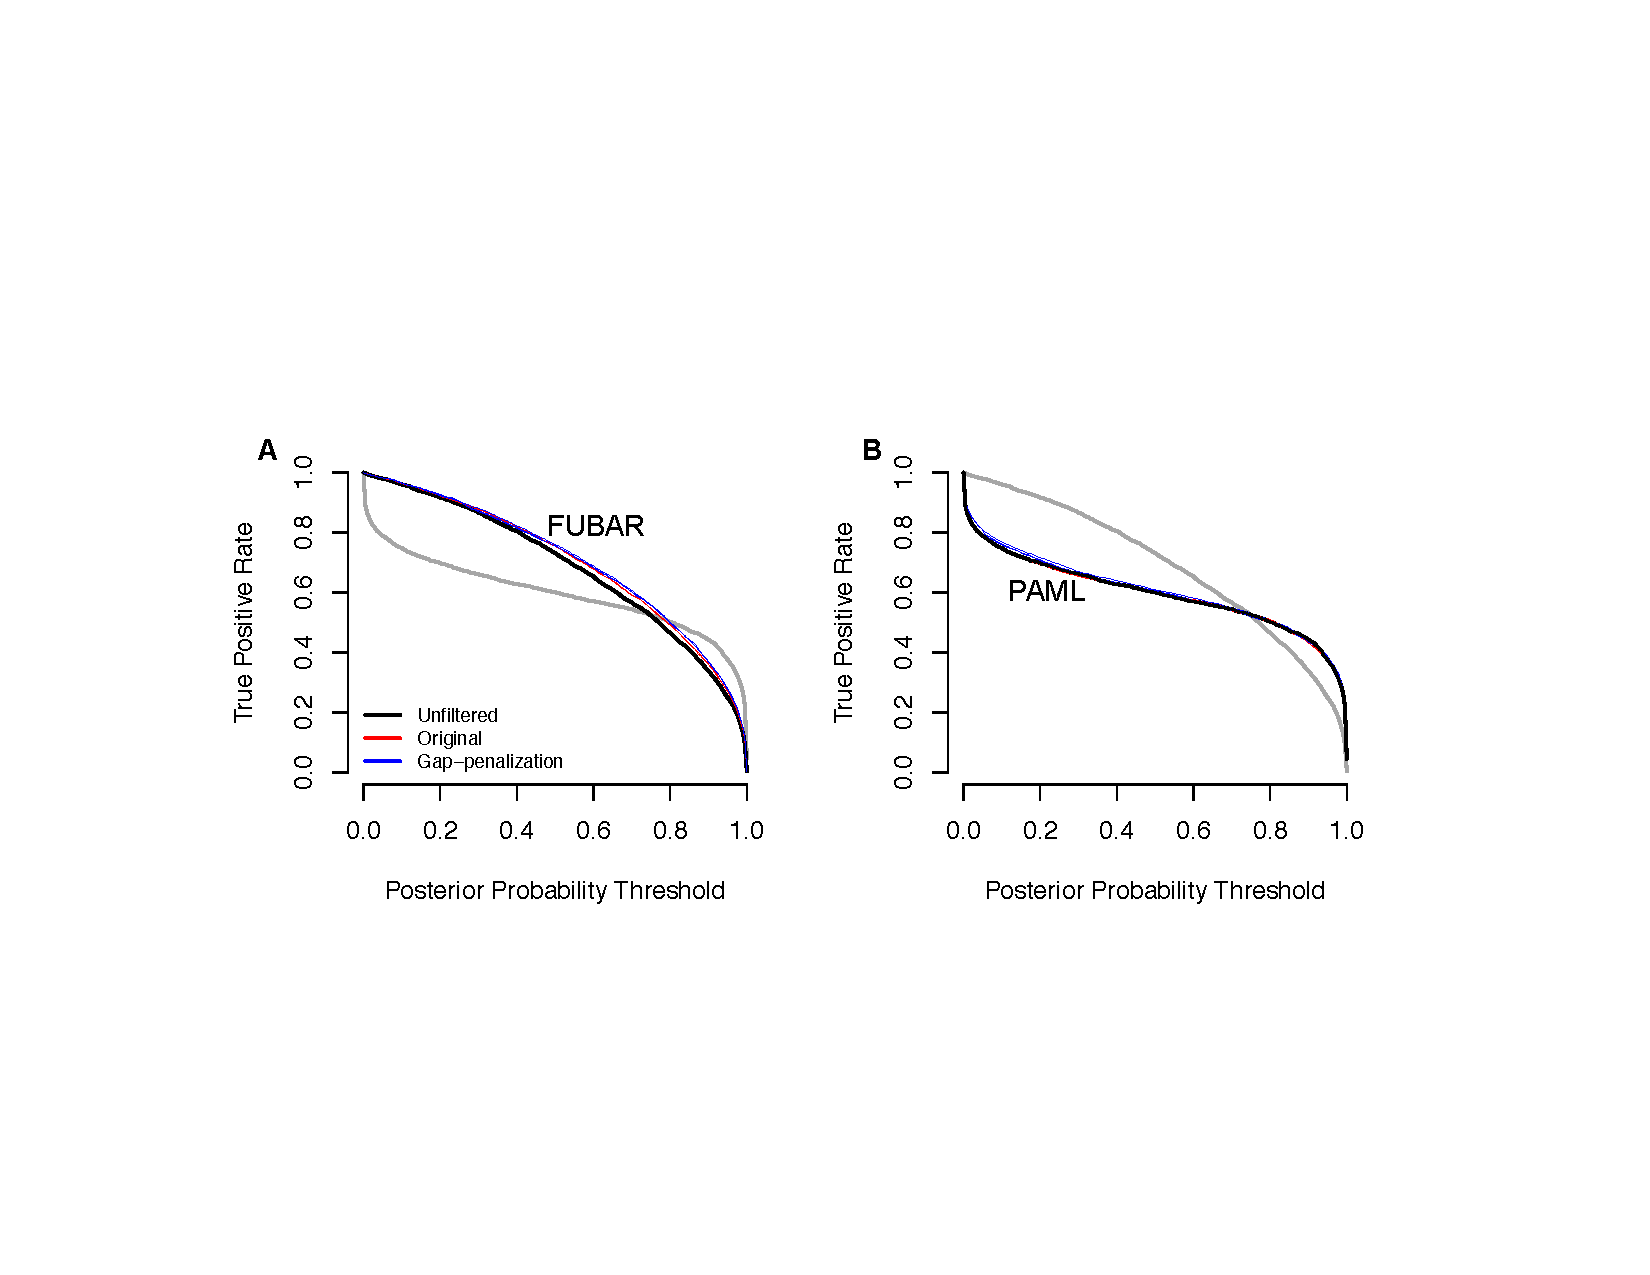
\includegraphics[width=7in]{Figures/fulltpr.pdf}}
\caption{\label{fulltpr} True positive rate against posterior probability threshold for calling positively selected sites, averaged across the 60-sequence simulation set. A) FUBAR in color with PAML results shown in grey. B) PAML in color with FUBAR results shown in grey. Filtered alignments behave similarly to unfiltered alignments across all posterior probabilities.}
\end{figure*}



\begin{table}[H]
\caption {\label{tab:penalmodel} Comparison of gap-penalization vs original normalization schemes on TPR of positive-selection inference.}
\begin{tabular}{l l l l l l}
\hline\noalign{\smallskip}
\multicolumn{1}{c}{Simulation Set} & \multicolumn{1}{c}{Method} & \multicolumn{1}{c}{Guidance} & \multicolumn{1}{c}{BMweights} & \multicolumn{1}{c}{PDweights} \\
\noalign{\smallskip}\hline\noalign{\smallskip}
11 taxa  & FUBAR & 0.001 (0.98\%) & $-1.76\times10^{-5}$ (-0.002\%) & 0.001 (0.95\%)\\
              & PAML & $-2.68\times10^{-4}$ (-0.31\%) & $2.57\times10^{-5}$ (0.03\%) & -0.001 (-1.50\%)\\
\hline
26 taxa   & FUBAR & 0.0032 (1.38\%) & 0.00040 (1.75\%) & 0.0018 (0.77\%)\\
              & PAML & \textbf{0.006}$^{\ast}$ (3.02\%) & \textbf{0.007}$^{\ast\ast}$ (3.32\%) & 0.006$^{\ast}$ (2.89\%) \\
\hline
60 taxa  & FUBAR & \textbf{0.010}$^{\ast}$ (2.67\%) & \textbf{0.012}$^{\ast\ast}$ (3.30\%)  & 0.005  (1.29\%)\\
              & PAML & -0.002 (-0.46\%) & 0.010 (2.23\%) & 0.008 (1.84\%) \\
\hline
158 taxa & FUBAR & 0.003 (0.79\%) & 0.002 (0.48\%) & 0.001 (0.28\%)\\
\hline
\end{tabular}
\newline
\textsc{note.}--- Significance levels: $^{\ast\ast} P < 0.01$; $^{\ast} P < 0.05$. Each column displays the magnitude of TPR difference between normalization schemes, represented as gap-penalization minus original, for each algorithm, respectively. Percentage changes from the original normalization scheme are shown in parentheses. All significance levels were corrected for multiple comparisons with the single-step method.
\end{table}


\begin{table}
\caption {\label{tab:casemodel} Effect of alignment filtering on TPR of positive-selection inference.}
\begin{tabular}{c c c l l l}
\hline\noalign{\smallskip}
& & & \multicolumn{3}{c}{Filtered TPR} \\
\cline{4-6}\noalign{\smallskip}
Simulation Set & Method & Unfiltered TPR & \multicolumn{1}{c}{GuidanceP} & \multicolumn{1}{c}{BMweightsP} & \multicolumn{1}{c}{PDweightsP} \\ 
\hline\noalign{\smallskip}
11 taxa  & FUBAR & 0.108 & 0.109  (1.04\%)   & 0.110  (1.86\%)  & 0.110  (1.37\%)        \\
              & PAML &  0.087 & 0.088  (0.49\%) &  0.088  (0.83\%)   & 0.088  (0.79\%)        \\
\hline
26 taxa   & FUBAR &  0.229 & 0.232 (1.54\%)  & 0.233 (1.83\%) & 0.233 (1.91\%)         \\
              & PAML & 0.194 & \textbf{0.204} (4.87\%)$^{\ast}$ & \textbf{0.203} (4.56\%)$^{\ast}$ & \textbf{0.203} (4.58\%)$^{\ast}$   \\
\hline
60 taxa  & FUBAR & 0.345 & \textbf{0.379} (9.92\%)$^{\ast\ast}$ & \textbf{0.377} (9.31\%)$^{\ast\ast}$ & \textbf{0.375} (8.75\%)$^{\ast\ast}$  \\
              & PAML & 0.447 & 0.447 (0.19\%) & 0.440 (-1.43\%) & 0.445 (-0.30\%) \\
\hline
158 taxa & FUBAR & 0.374 & \textbf{0.388} (3.89\%)$^{\ast\ast}$ & \textbf{0.387} (3.68\%)$^{\ast\ast}$ & \textbf{0.387} (3.47\%)$^{\ast\ast}$  \\
\hline
\end{tabular}
\newline
\textsc{note.}--- Significance levels: $^{\ast\ast} P < 1\times10^{-5}$; $^{\ast} P < 1\times10^{-4}$. \textit{Unfiltered TPR}: average true positive rate (TPR) for unfiltered alignments; \textit{Filtered TPR}: average true positive rate (TPR) for alignments filtered with each respective algorithm, with percent change from unfiltered alignment shown in parentheses. All significance levels are relative to the given simulation set's unfiltered alignment. We detected no significant TPR differences among filters tested within sequence simulation sets. All significance levels were corrected for multiple comparisons with the single-step method.
\end{table}



\begin{table}
\caption {\label{tab:cutoffs} Effect of masking cutoff on TPR of positive-selection inference.}
\begin{tabular}{c c c c}
\hline\noalign{\smallskip}
Simulation Set & 0.5 TPR & 0.9 TPR & Percent TPR Decrease \\ 
\hline\noalign{\smallskip}
11 taxa & 0.104 & 0.104 & 4.99\%$^{\ast}$\\ 
26 taxa & 0.232 & 0.220 & 5.28\%$^{\ast\ast}$\\
60 taxa & 0.281 & 0.379 & 25.8\%$^{\ast\ast\ast}$\\
158 taxa & 0.374 & 0.388 & 3.57\%$^{\ast\ast\ast}$\\
\hline
\end{tabular}
\newline
\textsc{note.}--- Significance levels: $^{\ast\ast\ast} P < 1\times10^{-6}$; $^{\ast\ast} P < 1\times10^{-5}$; $^{\ast\ast} P < 1\times10^{-3}$. 

\textit{0.5 TPR}: average TPR for alignments masked at a cutoff of 0.5 with GuidanceP; \textit{0.9 TPR}: average TPR for alignments masked at a cutoff of 0.9 with GuidanceP; \textit{Percent TPR Decrease} average percent decrease in TPR recovered between alignments masked at cutoffs of 0.5 and 0.9. All significance levels were corrected for multiple comparisons with the single-step method.
\end{table}


\bibliographystyle{MBE}
\bibliography{citations}	

\end{document}